\chapter{Fundamentação teórica} \label{cha:fundteo}

\section{Amplificadores de potência} \label{sec:fundteo-pa}

Em sistemas de comunicação sem fio, os amplificadores de potência atuam após o processo de geração e modulação do sinal a ser transmitido e diretamente à frente da antena. Seu papel é amplificar a potência dos sinais gerados de forma que a transmissão por meio do ar seja efetiva, visto que a potência do sinal é relacionada à distância na qual o sinal transmitido pode ser captado e interpretado com clareza \cite{raychaudhuri_frontiers_2012}.

Alimentado por uma potência maior do que a presente nos sinais de entrada, o amplificador de potência apresenta um comportamento não-linear ao operar em sua região de maior eficiência, ou seja, na sua região mais próxima da sua potência de alimentação \cite{cripps_rf_2006}.

A \autoref{fig:model-pa-p} mostra um modelo do amplificador de potência com as potências de entrada, de alimentação, dissipada e de saída representadas.

\imagem{Modelo simplificado de PA com as potências}{
\resizebox{0.6\textwidth}{!}{
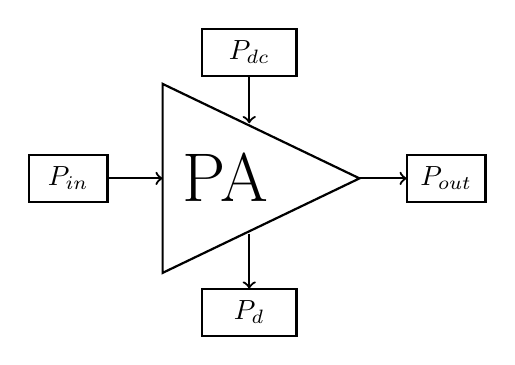
\begin{tikzpicture}[thick]      
      \draw  (-2.5,1.7)  -- (-2.5,-0.7) -- (0,0.5) -- cycle;
      \draw[->] (-3.2,0.5) -- (-2.5,0.5);
      \node at (-1.7,0.5) {\Huge PA};
      \draw[->] (-1.4,1.8) -- (-1.4,1.2);
      \draw[->] (-1.4,-0.2) -- (-1.4,-0.9);
      \draw[->] (0,0.5) -- (0.6,0.5);
      \draw  (-2,2.4) rectangle node {$P_{dc}$} (-0.8,1.8);
      \draw  (-4.2,0.8) rectangle node {$P_{in}$} (-3.2,0.2);
      \draw  (-0.8,-1.5) rectangle node {$P_{d}$}(-2,-0.9);
      \draw  (0.6,0.8) rectangle node {$P_{out}$} (1.6,0.2);
\end{tikzpicture}}
\label{fig:model-pa-p}
}{O autor}{fig:model-pa-p}{}{Modelo de PA com as potências de entrada $P_{in}$, de saída $P_{out}$, de alimentação $P_{dc}$ e a perda $P_{d}$ indicadas.}

A eficiência \criarsimbolo{$\eta$}{Eficiência}\label{item:efi} pode ser caracterizada como a razão entre a potência de saída e a potência de alimentação, conforme a equação \ref{eq:resultado}, e num caso ideal seria máxima na região de maior potência de saída. No entanto, a região com a máxima potência de saída é justamente a região de funcionamento não-linear do amplificador de potência e são necessárias técnicas para compensar essa não linearidade presente.

\begin{align}
\eta = \frac{P_{out}}P_{dc}
\label{eq:resultado}
\end{align}

\section{Linearização do PA} \label{sec:fundteo-line}
A linearização é o processo necessário para compensar as não linearidades presentes, ocorrendo através da passagem dos sinais a serem transmitidos por uma função que possui o comportamento inverso ao comportamento do PA analisado \cite{kenington_high-linearity_2000}. Na \autoref{fig:linearizacao} está presente um exemplo simplificado desse processo, no qual o sinal S passa por um pré-distorcedor digital (DPD) que possui o perfil inverso ao perfil do PA, desconsiderando-se o ganho K, e após este processo o sinal resultante é distorcido e amplificado pelo PA. Como o sinal DPD(S) foi anteriormente pré-distorcido, temos como saída dos blocos em cascata um sinal que sofreu somente uma amplificação.

\imagem{Cascata DPD-PA}{
\resizebox{0.8\textwidth}{!}{
\label{fig:linearizacao}
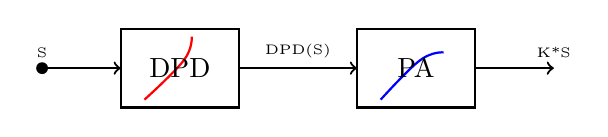
\begin{tikzpicture}[->,thick]
		\draw[-,blue]  plot[smooth, tension=.7] coordinates {(0.8,0.1) (1.3,0.6) (1.6,0.7)};
		\draw[-,red]  plot[smooth, tension=.7] coordinates {(-2.2,0.1) (-1.7,0.6) (-1.6,0.9)};
        \draw  (-2.5,1) rectangle node {DPD} (-1,0);
        \draw  (0.5,1) rectangle node {PA} (2,0);
        \draw (2,0.5) --  (3,0.5) node[above] {\tiny K*S};
        \draw (-1,0.5) -- node[above] {\tiny DPD(S)} (0.5,0.5);
        \draw (-3.5,0.5) node[above] {\tiny S} -- (-2.5,0.5);
        \node[circle, fill,minimum size=1.5mm,inner sep=0pt,outer sep=0pt] at (-3.5,0.5) {};
\end{tikzpicture}
}
}{O autor}{fig:linearizacao}{}{Cascata DPD-PA para o processo de amplificação do sinal S por um ganho K, mantendo-se a linearidade de S.}

A construção da função inversa do PA através de técnicas de caixa preta, por possuir um perfil inverso ao mesmo, possui uma complexidade, tanto no processo de treinamento como na quantidade de coeficientes do modelo, que pode ser relacionada ao quão não-linear é a curva do PA estudado. Isso se traduz em um maior esforço nas etapas de modelagem e de treinamento dos modelos inversos para se obter resultados com igual grau de confiança.

\section{Bijetividade e função inversa} \label{sec:fundteo-bije}
Para se compreender o quão não-linear é um modelo de PA, utiliza-se o conceito de bijetividade e da separação do modelo em suas regiões monotônica e não-monotônica.

A bijetividade é uma característica necessária para a existência de uma inversa única, seja esta analítica ou numérica \cite{weisstein}. Sabe-se que a existência de uma função inversa $f^{-1}$, conforme exemplificado na equação \ref{eq:equacao_generica} e na \autoref{fig:fun_generica}, necessita que para cada elemento do contradomínio de $f$ exista um e somente um elemento no domínio de $f$.

\begin{align}
f(f^{-1}(x)) = x
\label{eq:equacao_generica}
\end{align}

\imagem{Função genérica e sua inversa}{
\label{fig:fun_generica}
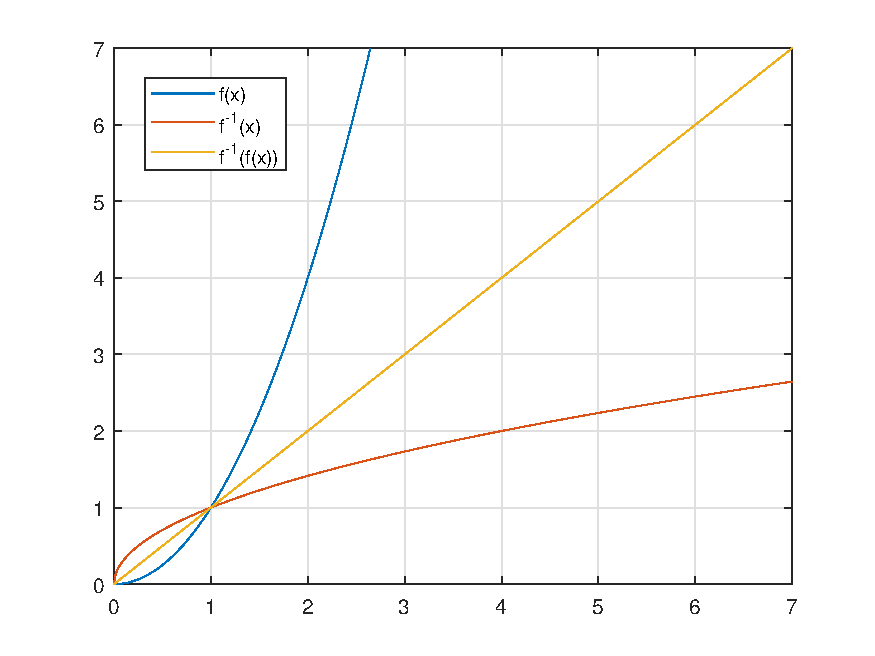
\includegraphics[width = 0.8\textwidth]{fig/Inversa-eps-converted-to.pdf}
}{O autor}{fig:fun_generica}{}{Função $f(x)$, sua inversa $f^{-1}(x)$ e a composição $f^{-1}(f(x))$ representadas de forma gráfica.}

Essa relação pode ser facilmente observada através da \autoref{fig:bijetividade}, sendo o primeiro conjunto o domínio da função $f$ e o segundo conjunto o contradomínio desta, enquanto para a função $f^{-1}$ essa relação se inverte.

\imagem{Função bijetiva e sua inversa}{
\resizebox{0.8\textwidth}{!}{
\label{fig:bijetividade}

\begin{tikzpicture}[->,thick]
 \node (a) at (0,0.5) {$A$};
 \node (b) at (0,0) {$B$};
 \node (c) at (0,-0.5) {$C$};
 \node[draw, ellipse, minimum height=2.5cm,minimum width=1.5cm, fit=(a) (b) (c)] {};
  
\node (d) at (2,0.5) {$X$};
\node (e) at (2,0) {$Y$};
\node (f) at (2,-0.5) {$Z$};
\node[draw, ellipse, minimum height=2.5cm,minimum width=1.5cm, fit=(d) (e) (f)] {};

\draw  (c) edge (f);
\draw  (b) edge (e);
\draw  (a) edge (d);
\node at (1,1.5) {$f$};

\node (a) at (4,0.5) {$X$};
\node (b) at (4,0) {$Y$};
\node (c) at (4,-0.5) {$Z$};
\node[draw, ellipse, minimum height=2.5cm,minimum width=1.5cm, fit=(a) (b) (c)] {};
  
\node (d) at (6,0.5) {$A$};
\node (e) at (6,0) {$B$};
\node (f) at (6,-0.5) {$C$};
\node[draw, ellipse, minimum height=2.5cm,minimum width=1.5cm, fit=(d) (e) (f)] {};

\draw  (c) edge (f);
\draw  (b) edge (e);
\draw  (a) edge (d);
\node at (5,1.5) {$f^{-1}$};

\end{tikzpicture}
}
}{O autor}{fig:bijetividade}{}{Função bijetiva $f(x)$, sua inversa $f^{-1}(x)$ e a composição $f^{-1}(f(x))$ representadas através da relação entre conjuntos.}

A função do PA, portanto, desta perspectiva, não é bijetiva, pois apresenta uma região não-monotônica na qual para diferentes elementos no contradomínio existem dois ou mais elementos no domínio desta, o que pode ser visto na \autoref{fig:perfil_pa}. Nesta figura também é possível observar que a maior parte do modelo do PA é monotônica e crescente, ou seja, desconsiderando-se os efeitos de memória, essa parte da função é passível de possuir uma inversa.

\imagemH{Perfil de um PA}{
\label{fig:perfil_pa}
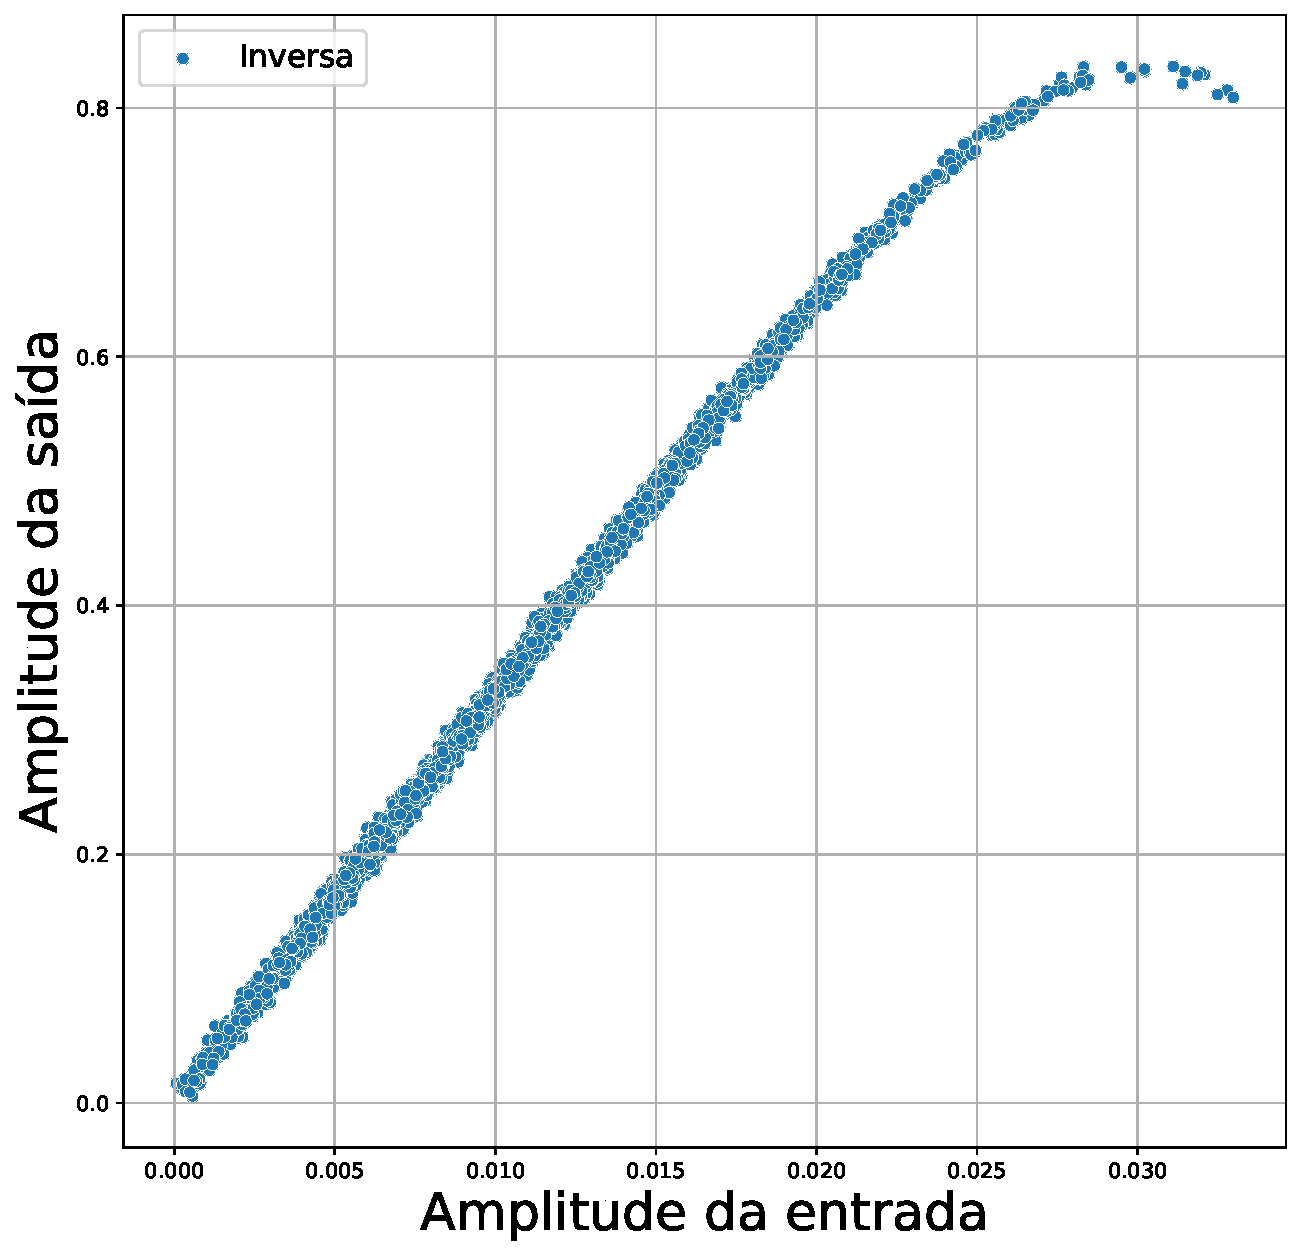
\includegraphics[width = 0.8\textwidth]{fig/modelo_pa.pdf}
}{O autor}{fig:perfil_pa}{}{Perfil de um PA, com os valores normalizados, mostrando sua região não-linear na região com entradas e saídas com maiores amplitudes.}

Apesar da função inversa do PA não ser única, a presença de elementos de memória que afetam o estado atual se torna uma condição de contorno para determinar o valor correto para a inversa em razão das entradas atuais e passadas. Na modelagem da inversa do PA, por meio da topologia presente neste trabalho, essa informação se torna implícita no modelo de caixa preta utilizado.

\section{Distorção digital} \label{sec:fundteo-distor}
O termo utilizado para o processo de linearização de PAs é distorção digital, tendo em vista que os sinais a serem enviados são distorcidos pela inversa do PA ainda na etapa digital do processamento, antes de serem convertidos em sinais analógicos. Sendo um modo de conciliar a eficiência e a linearidade do PA, os distorcedores digitais podem ser separados em duas categorias básicas: Os pré-distorcedores digitais (DPDs) e os pós-distorcedores digitais (PoDs).

Um pré-distorcedor digital é um sistema pré-inverso, que distorce o sinal antes deste passar pela PA, conforme a \autoref{fig:dpd_cascata}. Enquanto o pós-distorcedor digital (PoD) é uma pós-inversa, que distorce o sinal após sua passagem pelo PA, como mostrado na \autoref{fig:pod_cascata}. Embora ambas sejam funções inversas do PA, o uso de PoD é inviável na prática, devido às altas potências presentes na saída do PA.

\imagem{Cascata DPD-PA com sinal desconhecido}{
\resizebox{0.8\textwidth}{!}{
\label{fig:dpd_cascata}
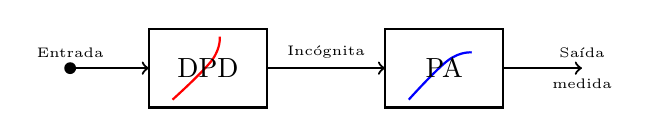
\begin{tikzpicture}[->,thick]
		\draw[-,blue]  plot[smooth, tension=.7] coordinates {(0.8,0.1) (1.3,0.6) (1.6,0.7)};
		\draw[-,red]  plot[smooth, tension=.7] coordinates {(-2.2,0.1) (-1.7,0.6) (-1.6,0.9)};
        \draw  (-2.5,1) rectangle node {DPD} (-1,0);
        \draw  (0.5,1) rectangle node {PA} (2,0);
        \draw (2,0.5) --  (3,0.5) node[above] {\tiny Saída} node[below] {\tiny medida};
        \draw (-1,0.5) -- node[above] {\tiny Incógnita} (0.5,0.5);
        \draw (-3.5,0.5) node[above] {\tiny Entrada} -- (-2.5,0.5);
        \node[circle, fill,minimum size=1.5mm,inner sep=0pt,outer sep=0pt] at (-3.5,0.5) {};
\end{tikzpicture}
}
}{O autor}{fig:dpd_cascata}{}{Cascata DPD-PA ilustrando as distorções sofridas pelo sinal de entrada, no qual o sinal intermediário é desconhecido.}

\imagem{Cascata PA-PoD}{
\resizebox{0.8\textwidth}{!}{
\label{fig:pod_cascata}
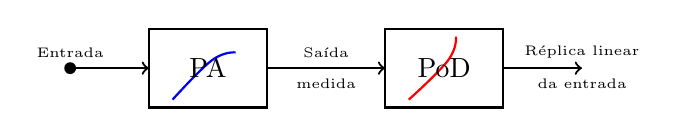
\begin{tikzpicture}[->,thick]
        \draw[-,blue]  plot[smooth, tension=.7] coordinates {(-2.2,-1.4) (-1.7,-0.9) (-1.4,-0.8)};
		\draw[-,red]  plot[smooth, tension=.7] coordinates {(0.8,-1.4) (1.3,-0.9) (1.4,-0.6)};
        \draw  (-2.5,-0.5) rectangle node {PA} (-1,-1.5);
        \draw  (0.5,-0.5) rectangle node {PoD} (2,-1.5);
        \draw (2,-1) -- (3,-1) node[above] {\tiny Réplica linear} node[below] {\tiny da entrada};
        \draw (-3.5,-1) node[above] {\tiny Entrada} -- (-2.5,-1);
        \draw (-1,-1) -- node[above] {\tiny Saída} node[below] {\tiny medida} (0.5,-1);
        \node[circle, fill,minimum size=1.5mm,inner sep=0pt,outer sep=0pt] at (-3.5,-1) {};
\end{tikzpicture}
}
}{O autor}{fig:pod_cascata}{}{Cascata PA-PoD ilustrando as distorções sofridas pelo sinal de entrada, no qual o sinal intermediário é a saída conhecida do PA.}

Para os projetos do DPD e PoD, dois conjuntos de entradas e saídas medidas precisam estar disponíveis: um para o treinamento e outro para a validação. O projeto do PoD é uma modelagem computacional clássica, na qual todas as informações do PoD são conhecidas. As informações para o PoD são obtidas pela troca de papéis da entrada e da saída do PA. Entretanto, por causa de sua saída desconhecida, projetar um DPD requer uma maior complexidade em relação ao PoD.

No que concerne ao treinamento do DPD, para contornar o treinamento direto mais pesado do DPD, uma arquitetura para aprendizado indireto (ILA) é usualmente adotada. Na ILA, os parâmetros do modelo de PoD são primeiro identificados considerando-se um cenário mais clássico, no qual ambos os sinais de entrada e saída são conhecidos, e então os parâmetros são copiados para um modelo de DPD com a mesma topologia \cite{changsoo_eun_new_1997}.

No entanto, uma validação de DPD mais confiável exige o seu uso como um modelo pré-inverso. Por essa razão, na literatura é usualmente requerida uma nova medição do PA após o treinamento, como visto em \cite{8891388}. Neste método, uma sequência pré-distorcida é aplicada como a entrada do PA para a medição de sua saída. A saída do PA é então comparada com o sinal de entrada do DPD e o erro entre a entrada da cascata e o sinal de saída é calculado.

\section{Modelagem} \label{sec:fundteo-model}
O treinamento e a validação dos PAs e suas inversas fazem parte do campo da modelagem computacional, no qual estes sistemas são representados por modelos matemáticos que simulam seu comportamento. Neste trabalho uma abordagem caixa preta foi utilizada, que possui como característica usar um modelo cujos coeficientes não possuem uma relação física com o funcionamento do sistema e busca somente reproduzir seu comportamento \cite{8882211}.

Outra opção seriam os modelos conhecidos como caixa branca, nos quais as funções presentes no modelo fazem referência direta ao comportamento do sistema ou a seus componentes internos. Estes modelos possuem como vantagem o fato de seus coeficientes possuírem significados físicos. No entanto, o seu desenvolvimento pode ser mais demorado e sua utilização só é permitida para representar sistemas físicos cujo comportamento é bem conhecido \cite{8882211}.

No caso das funções inversas, por não serem circuitos eletrônicos previamente existentes, os modelos caixa branca não são uma opção viável e o comportamento das mesmas deve ser reproduzido através de modelos caixa preta.

Em ambos os casos, uma das principais funções de um modelo é prover um substituto às medições físicas, decorrente do fato das medições físicas onerarem em tempo, recursos e espaço. A utilização de modelos permite a realização de análises de forma mais prática.
Dentre as diversas técnicas de modelagem caixa preta existentes, como as séries polinomiais, foi escolhido para este trabalho o uso de redes neurais artificiais do tipo perceptron de multicamada (MLP) em uma topologia específica para valores complexos.

